% DeltaCache System Architecture - TikZ Figure
% For IJCNN 2025 Paper
% Compile with: pdflatex architecture.tex

\documentclass[tikz,border=5pt]{standalone}
\usepackage{tikz}
\usetikzlibrary{shapes.geometric, arrows.meta, positioning, fit, backgrounds, calc, decorations.pathreplacing, shadows.blur, patterns}

% Color scheme - Professional blue-orange theme
\definecolor{primaryblue}{RGB}{41, 98, 255}
\definecolor{secondaryblue}{RGB}{66, 133, 244}
\definecolor{lightblue}{RGB}{232, 240, 254}
\definecolor{accentorange}{RGB}{255, 152, 0}
\definecolor{lightorange}{RGB}{255, 243, 224}
\definecolor{successgreen}{RGB}{52, 168, 83}
\definecolor{lightgreen}{RGB}{232, 245, 233}
\definecolor{warningred}{RGB}{234, 67, 53}
\definecolor{neutralgray}{RGB}{95, 99, 104}
\definecolor{lightgray}{RGB}{248, 249, 250}
\definecolor{darktext}{RGB}{32, 33, 36}
\definecolor{gpucolor}{RGB}{118, 185, 0}
\definecolor{cpucolor}{RGB}{156, 39, 176}

\begin{document}
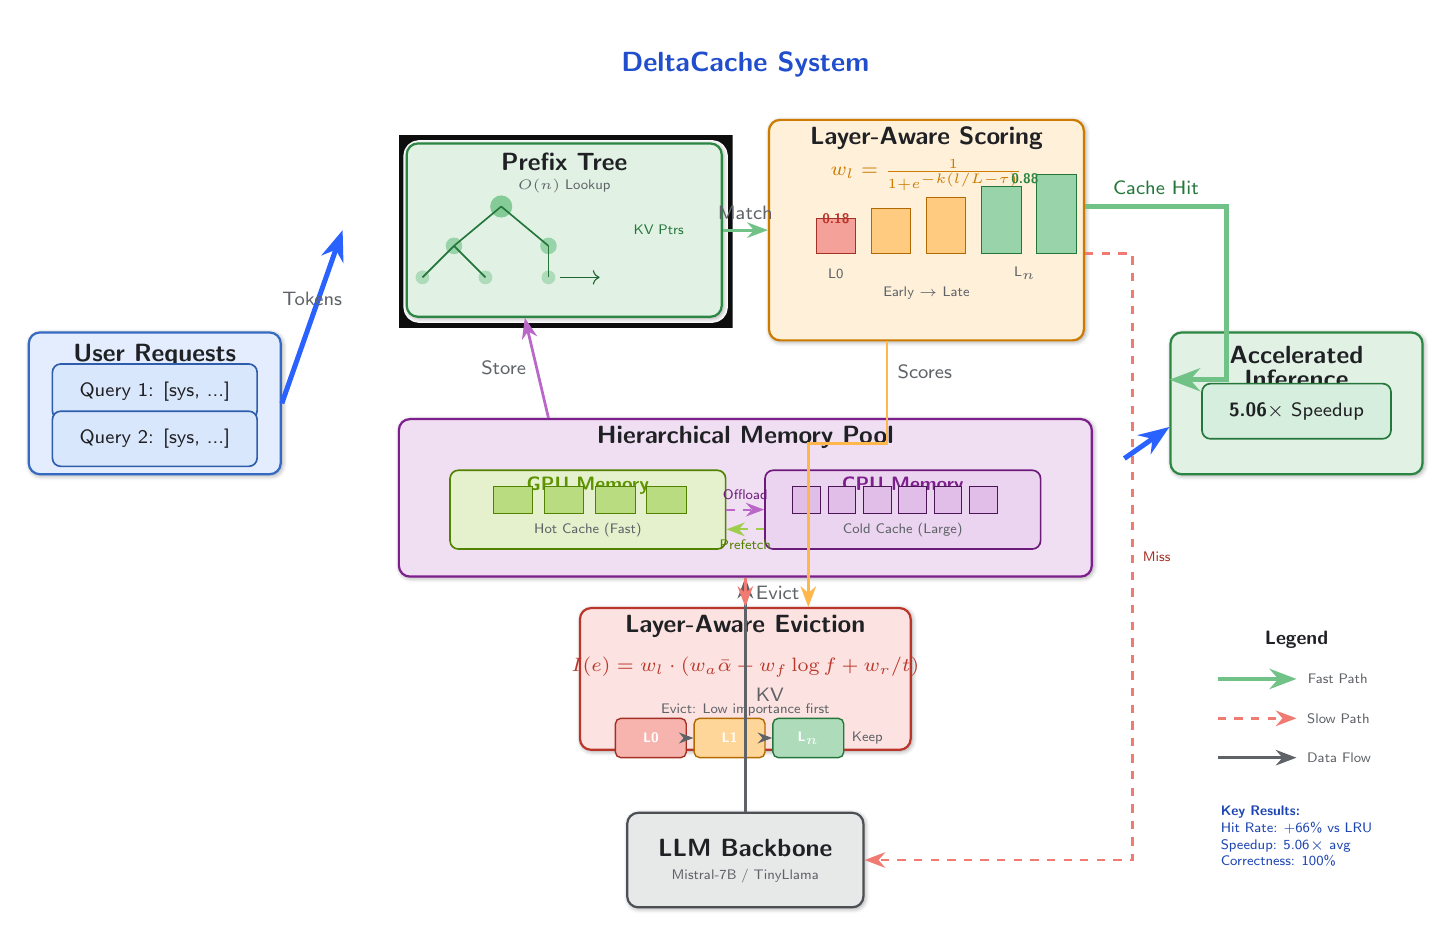
\begin{tikzpicture}[
    % Node styles
    component/.style={
        rectangle,
        rounded corners=4pt,
        minimum width=2.8cm,
        minimum height=1cm,
        draw=#1!80!black,
        fill=#1!15,
        line width=0.8pt,
        font=\small\sffamily,
        text=darktext,
        blur shadow={shadow blur steps=5, shadow xshift=0.5pt, shadow yshift=-0.5pt}
    },
    mainbox/.style={
        rectangle,
        rounded corners=8pt,
        draw=#1!70!black,
        fill=#1!8,
        line width=1.2pt,
        inner sep=12pt
    },
    smallbox/.style={
        rectangle,
        rounded corners=3pt,
        minimum width=1.8cm,
        minimum height=0.7cm,
        draw=#1!70!black,
        fill=#1!20,
        line width=0.6pt,
        font=\scriptsize\sffamily,
        text=darktext
    },
    layerbox/.style={
        rectangle,
        rounded corners=2pt,
        minimum width=0.9cm,
        minimum height=0.5cm,
        draw=#1!70!black,
        fill=#1!40,
        line width=0.5pt,
        font=\tiny\sffamily\bfseries,
        text=white
    },
    arrow/.style={
        ->,
        >=Stealth,
        line width=1pt,
        #1
    },
    dataarrow/.style={
        ->,
        >=Stealth,
        line width=1.5pt,
        primaryblue
    },
    bigarrow/.style={
        ->,
        >=Stealth,
        line width=2pt,
        #1
    },
    label/.style={
        font=\scriptsize\sffamily,
        text=neutralgray
    },
    title/.style={
        font=\small\sffamily\bfseries,
        text=darktext
    },
    subtitle/.style={
        font=\tiny\sffamily,
        text=neutralgray
    }
]

% ============================================
% Input Section (Left)
% ============================================
\node[component=secondaryblue, minimum width=3.2cm, minimum height=1.8cm] (input) at (0, 0) {};
\node[title] at (input.north) [yshift=-0.3cm] {User Requests};
\node[subtitle] at (input.south) [yshift=0.4cm] {Token Sequences};

% Query examples inside input
\node[smallbox=secondaryblue, minimum width=2.6cm] (q1) at ($(input.center)+(0, 0.15)$) {Query 1: [sys, ...]};
\node[smallbox=secondaryblue, minimum width=2.6cm] (q2) at ($(input.center)+(0, -0.45)$) {Query 2: [sys, ...]};

% ============================================
% Main DeltaCache System (Center)
% ============================================
\begin{scope}[on background layer]
    \node[mainbox=primaryblue, minimum width=10cm, minimum height=9.5cm] (mainsystem) at (7.5, 0) {};
\end{scope}
\node[font=\normalsize\sffamily\bfseries, text=primaryblue!80!black] at (7.5, 4.3) {\textsc{DeltaCache} System};

% --- Prefix Tree Module ---
\node[component=successgreen, minimum width=4cm, minimum height=2.2cm] (prefixtree) at (5.2, 2.2) {};
\node[title] at (prefixtree.north) [yshift=-0.25cm] {Prefix Tree};
\node[subtitle] at (prefixtree.north) [yshift=-0.55cm] {$O(n)$ Lookup};

% Tree structure visualization
\coordinate (root) at ($(prefixtree.center)+(-0.8, 0.3)$);
\coordinate (child1) at ($(root)+(-0.6, -0.5)$);
\coordinate (child2) at ($(root)+(0.6, -0.5)$);
\coordinate (leaf1) at ($(child1)+(-0.4, -0.4)$);
\coordinate (leaf2) at ($(child1)+(0.4, -0.4)$);
\coordinate (leaf3) at ($(child2)+(0, -0.4)$);

\fill[successgreen!60] (root) circle (4pt);
\fill[successgreen!50] (child1) circle (3pt);
\fill[successgreen!50] (child2) circle (3pt);
\fill[successgreen!40] (leaf1) circle (2.5pt);
\fill[successgreen!40] (leaf2) circle (2.5pt);
\fill[successgreen!40] (leaf3) circle (2.5pt);

\draw[successgreen!70!black, line width=0.6pt] (root) -- (child1);
\draw[successgreen!70!black, line width=0.6pt] (root) -- (child2);
\draw[successgreen!70!black, line width=0.6pt] (child1) -- (leaf1);
\draw[successgreen!70!black, line width=0.6pt] (child1) -- (leaf2);
\draw[successgreen!70!black, line width=0.6pt] (child2) -- (leaf3);

% KV pointer annotation
\node[font=\tiny\sffamily, text=successgreen!70!black] at ($(prefixtree.center)+(1.2, 0)$) {KV Ptrs};
\draw[->, successgreen!60!black, line width=0.4pt] ($(leaf3)+(0.15, 0)$) -- ++(0.5, 0);

% --- Layer-Aware Importance Module ---
\node[component=accentorange, minimum width=4cm, minimum height=2.8cm] (importance) at (9.8, 2.2) {};
\node[title] at (importance.north) [yshift=-0.25cm] {Layer-Aware Scoring};

% Sigmoid formula
\node[font=\scriptsize, text=accentorange!80!black] at ($(importance.center)+(0, 0.7)$) {$w_l = \frac{1}{1 + e^{-k(l/L - \tau)}}$};

% Layer visualization with gradient
\foreach \i/\w/\c in {0/0.18/warningred, 1/0.35/accentorange, 2/0.52/accentorange, 3/0.70/successgreen, 4/0.88/successgreen} {
    \pgfmathsetmacro{\xpos}{-1.4 + \i * 0.7}
    \pgfmathsetmacro{\height}{0.3 + \w * 0.8}
    \fill[\c!50] ($(importance.center)+(\xpos, -0.3)$) rectangle ++(0.5, \height);
    \draw[\c!70!black, line width=0.3pt] ($(importance.center)+(\xpos, -0.3)$) rectangle ++(0.5, \height);
}

% Layer labels
\node[font=\tiny\sffamily, text=neutralgray] at ($(importance.center)+(-1.15, -0.55)$) {L0};
\node[font=\tiny\sffamily, text=neutralgray] at ($(importance.center)+(1.25, -0.55)$) {L$_n$};
\node[font=\tiny\sffamily, text=neutralgray] at ($(importance.center)+(0, -0.8)$) {Early $\rightarrow$ Late};

% Weight annotation
\node[font=\tiny\sffamily\bfseries, text=warningred!80!black] at ($(importance.center)+(-1.15, 0.15)$) {0.18};
\node[font=\tiny\sffamily\bfseries, text=successgreen!80!black] at ($(importance.center)+(1.25, 0.65)$) {0.88};

% --- Memory Pool Module ---
\node[component=cpucolor, minimum width=8.8cm, minimum height=2cm] (mempool) at (7.5, -1.2) {};
\node[title] at (mempool.north) [yshift=-0.25cm] {Hierarchical Memory Pool};

% GPU section
\node[smallbox=gpucolor, minimum width=3.5cm, minimum height=1cm] (gpu) at ($(mempool.center)+(-2, -0.15)$) {};
\node[font=\scriptsize\sffamily\bfseries, text=gpucolor!80!black] at (gpu.north) [yshift=-0.2cm] {GPU Memory};
\node[font=\tiny\sffamily, text=neutralgray] at (gpu.south) [yshift=0.25cm] {Hot Cache (Fast)};

% GPU blocks
\foreach \i in {0, 1, 2, 3} {
    \fill[gpucolor!50] ($(gpu.center)+(-1.2 + \i*0.65, -0.05)$) rectangle ++(0.5, 0.35);
    \draw[gpucolor!70!black, line width=0.3pt] ($(gpu.center)+(-1.2 + \i*0.65, -0.05)$) rectangle ++(0.5, 0.35);
}

% CPU section
\node[smallbox=cpucolor, minimum width=3.5cm, minimum height=1cm] (cpu) at ($(mempool.center)+(2, -0.15)$) {};
\node[font=\scriptsize\sffamily\bfseries, text=cpucolor!80!black] at (cpu.north) [yshift=-0.2cm] {CPU Memory};
\node[font=\tiny\sffamily, text=neutralgray] at (cpu.south) [yshift=0.25cm] {Cold Cache (Large)};

% CPU blocks
\foreach \i in {0, 1, 2, 3, 4, 5} {
    \fill[cpucolor!30] ($(cpu.center)+(-1.4 + \i*0.45, -0.05)$) rectangle ++(0.35, 0.35);
    \draw[cpucolor!50!black, line width=0.3pt] ($(cpu.center)+(-1.4 + \i*0.45, -0.05)$) rectangle ++(0.35, 0.35);
}

% Offload arrow between GPU and CPU
\draw[arrow=cpucolor!70, line width=0.8pt, dashed] ($(gpu.east)+(0, 0)$) -- node[above, font=\tiny\sffamily, text=cpucolor!70!black] {Offload} ($(cpu.west)+(0, 0)$);
\draw[arrow=gpucolor!70, line width=0.8pt, dashed] ($(cpu.west)+(0, -0.25)$) -- node[below, font=\tiny\sffamily, text=gpucolor!70!black] {Prefetch} ($(gpu.east)+(0, -0.25)$);

% --- Eviction Policy Module ---
\node[component=warningred, minimum width=4.2cm, minimum height=1.8cm] (eviction) at (7.5, -3.5) {};
\node[title] at (eviction.north) [yshift=-0.25cm] {Layer-Aware Eviction};

% Importance formula
\node[font=\scriptsize, text=warningred!80!black] at ($(eviction.center)+(0, 0.15)$) {$I(e) = w_l \cdot (w_a \bar{\alpha} + w_f \log f + w_r / t)$};

% Policy comparison
\node[font=\tiny\sffamily, text=neutralgray] at ($(eviction.center)+(0, -0.4)$) {Evict: Low importance first};

% Small layer icons showing eviction priority
\node[layerbox=warningred] (ev1) at ($(eviction.center)+(-1.2, -0.75)$) {L0};
\node[layerbox=accentorange] (ev2) at ($(eviction.center)+(-0.2, -0.75)$) {L1};
\node[layerbox=successgreen] (ev3) at ($(eviction.center)+(0.8, -0.75)$) {L$_n$};
\draw[arrow=neutralgray, line width=0.5pt] (ev1.east) -- (ev2.west);
\draw[arrow=neutralgray, line width=0.5pt] (ev2.east) -- (ev3.west);
\node[font=\tiny\sffamily, text=neutralgray] at ($(eviction.center)+(1.55, -0.75)$) {Keep};

% ============================================
% Output Section (Right)
% ============================================
\node[component=successgreen, minimum width=3.2cm, minimum height=1.8cm] (output) at (14.5, 0) {};
\node[title] at (output.north) [yshift=-0.3cm] {Accelerated};
\node[title] at (output.north) [yshift=-0.6cm] {Inference};

% Speedup indicator
\node[smallbox=successgreen, minimum width=2.4cm] (speedup) at ($(output.center)+(0, -0.1)$) {\textbf{5.06$\times$} Speedup};

% ============================================
% Model Component (Bottom)
% ============================================
\node[component=neutralgray, minimum width=3cm, minimum height=1.2cm] (model) at (7.5, -5.8) {};
\node[title] at (model.center) [yshift=0.15cm] {LLM Backbone};
\node[subtitle] at (model.center) [yshift=-0.2cm] {Mistral-7B / TinyLlama};

% ============================================
% Arrows and Data Flow
% ============================================

% Input to system
\draw[dataarrow, line width=1.8pt] (input.east) -- node[above, label] {Tokens} ($(prefixtree.west)+(-0.8, 0)$);

% Prefix tree to importance
\draw[arrow=successgreen!70, line width=1pt] (prefixtree.east) -- node[above, label] {Match} (importance.west);

% Cache hit path (fast)
\draw[bigarrow=successgreen!70, line width=1.8pt] ($(importance.east)+(0, 0.3)$) -- node[above, font=\scriptsize\sffamily, text=successgreen!70!black] {Cache Hit} ++(1.8, 0) |- ($(output.west)+(0, 0.3)$);

% Cache miss path
\draw[arrow=warningred!70, line width=1pt, dashed] ($(importance.east)+(0, -0.3)$) -- ++(0.6, 0) |- node[right, font=\tiny\sffamily, text=warningred!70!black, pos=0.25] {Miss} (model.east);

% Model to memory pool
\draw[arrow=neutralgray, line width=1pt] (model.north) -- node[right, label] {KV} ($(mempool.south)+(0, 0)$);

% Memory pool to prefix tree
\draw[arrow=cpucolor!70, line width=1pt] ($(mempool.north)+(-2.5, 0)$) -- node[left, label] {Store} ($(prefixtree.south)+(-0.5, 0)$);

% Eviction from memory pool
\draw[arrow=warningred!70, line width=1pt] (mempool.south) -- node[right, label] {Evict} (eviction.north);

% Importance to eviction
\draw[arrow=accentorange!70, line width=1pt] ($(importance.south)+(-0.5, 0)$) -- node[right, label, pos=0.3] {Scores} ++(0, -1.3) -| ($(eviction.north)+(0.8, 0)$);

% System to output
\draw[dataarrow, line width=1.8pt] ($(mempool.east)+(0.4, 0.5)$) -- ($(output.west)+(0, -0.3)$);

% ============================================
% Legend
% ============================================
\node[font=\scriptsize\sffamily\bfseries, text=darktext] at (14.5, -3) {Legend};
\draw[bigarrow=successgreen!70, line width=1.5pt] (13.5, -3.5) -- ++(1, 0) node[right, font=\tiny\sffamily, text=neutralgray] {Fast Path};
\draw[arrow=warningred!70, line width=1pt, dashed] (13.5, -4) -- ++(1, 0) node[right, font=\tiny\sffamily, text=neutralgray] {Slow Path};
\draw[arrow=neutralgray, line width=1pt] (13.5, -4.5) -- ++(1, 0) node[right, font=\tiny\sffamily, text=neutralgray] {Data Flow};

% ============================================
% Key Metrics Annotation
% ============================================
\node[font=\tiny\sffamily, text=primaryblue!70!black, align=left] at (14.5, -5.5) {
    \textbf{Key Results:}\\
    Hit Rate: +66\% vs LRU\\
    Speedup: 5.06$\times$ avg\\
    Correctness: 100\%
};

\end{tikzpicture}
\end{document}
